\documentclass[conference]{IEEEtran}

\usepackage{hyperref}
\usepackage{graphicx}
\usepackage{fancyhdr}
%\usepackage{lastpage}
\usepackage{amsmath}
\usepackage{amscd}
\usepackage{color}
\usepackage{url}
%\usepackage{moreverb}
\usepackage{verbatim}
\usepackage{textcomp}
\usepackage{mathptmx}
\usepackage{dingbat}
\usepackage{pifont}
\usepackage{acronym}
\usepackage{algpseudocode}
\usepackage{algorithm}
\usepackage{supertabular}
\usepackage{listings}
\usepackage{threeparttable}
\usepackage{pdflscape}
\usepackage{array}
\usepackage{multirow}
\usepackage{subfigure}
\usepackage{array}

\usepackage[numbers,sort]{natbib}
\lstset{columns=flexible,showstringspaces=false}

\renewcommand{\algorithmiccomment}[1]{\hfill {\tt //} #1}
\newcommand{\tick}{\ding{52}}
\newcommand{\xmark}{\ding{56}}

\makeatletter
\newcommand{\thickhline}{%
    \noalign {\ifnum 0=`}\fi \hrule height 1pt
    \futurelet \reserved@a \@xhline
}
\newcolumntype{"}{@{\hskip\tabcolsep\vrule width 1pt\hskip\tabcolsep}}
\makeatother

\date{}
\begin{document}

\author{
\IEEEauthorblockN{Dimitris Mitropoulos,\IEEEauthorrefmark{1}
Panos Louridas,\IEEEauthorrefmark{2}
Michalis Polychronakis,\IEEEauthorrefmark{1}
and Angelos D. Keromytis\IEEEauthorrefmark{1}}
\IEEEauthorblockA{\IEEEauthorrefmark{1}
Network Security Lab\\
Department of Computer Scinence\\
Columbia University\\
\{dimitro, mikepo, angelos\}@cs.columbia.edu\\
\IEEEauthorrefmark{2}
Software Engineering and Security Lab\\
Department of Management Science and Technology\\
Athens University of Economics and Business\\
louridas@aueb.gr
}}

\title{SoK: The Evolution of Defenses Against Web Application Attacks}

\maketitle
\begin{abstract}

  Some of the most dangerous web application attacks, like Cross-Site
  Scripting and {\sc sql} injection, exploit the oversight of
  programmers that develop applications which may accept and process
  data of uncertain origin without appropriate validation and / or
  filtering. Such attacks, relying on source code injection
  vulnerabilities, have been constantly topping the lists of the
  various security bulletin providers despite the numerous
  countermeasures that have been proposed over the past 15 years.

  In this paper we systematize the existing knowledge regarding
  various defense mechanisms against source code injection by setting
  up a model that highlights the key weaknesses behind such attacks and
  helps us observe defenses from a common perspective.

  We then categorize and analyze the various defense mechanisms that
  have been developed. Our analysis is based on dimensions such as
  accuracy, performance, deployment, security and availability.
  Especially notable is accuracy, as our findings show that there are
  many defense mechanisms that are tested in a poor manner.
  In addition, we observe that there are mechanisms
  that can be bypassed by attackers that know how the mechanisms
  work.

  By comparing the existing defenses and identifying their common
  characteristics, we help: a) researchers and practitioners to choose
  or modify a mechanism according to their needs, and b) designers of
  new approaches in developing more efficient mechanisms.

\end{abstract}

\begin{IEEEkeywords}
Security and Protection, Application Security, Code injection Attacks,
Testing, Cross-Site Scripting.
\end{IEEEkeywords}

\IEEEpeerreviewmaketitle

\section{Introduction Remarks}

Web application attacks may involve security misconfigurations, broken
authentication and session management, or other issues. Some of the
most dangerous web application attacks are associated with the
processing of external input data that can contain malicious code, a
vulnerability known as code injection.

Such attacks include Cross-Site Scripting ({\sc xss})
attacks~\cite{SG07}, {\sc sql} injection attacks~\cite{RL12b},
Cross-Site Request Forgery ({\sc csrf}) attacks~\cite{LZRL09}, and
others. Attacks like these have been topping the vulnerability lists
of numerous bulletin providers like the Open Web Application Security
Project\footnote{\url{https://www.owasp.org/index.php/Category:OWASP_Top_Ten_Project}}
({\sc owasp}) and {\sc
  mitre}\footnote{\url{http://cwe.mitre.org/top25/}} for several
years. Consider the case of {\sc owasp}'s Top Ten project whose main
goal is to raise awareness about web application security by
identifying some of the most critical risks facing organizations. The
Top Ten project is popular, referenced by numerous researchers. In its
three consecutive Top Ten lists (2007, 2010, 2013), different
source code-driven injection attacks dominate the top five
positions. Malicious users find new ways~\cite{HNSHS12,DKH14}
to bypass defense mechanisms by using a variety of
techniques despite the numerous countermeasures
that are being introduced. Note that the number of systems developed
to counter {\sc sql} injection attacks until 2006 was more than
twenty~\cite{HVO06}. Since then the number has doubled. Researchers
have also indicated that the number of such attacks is steadily
increasing in recent years~\cite{SSL12}.

In this paper we initially show how the above attacks can be seen from
a {\it common perspective}. We achieve this by providing an
exploitation model that highlights the following fact: the majority of
the steps needed to perform application attacks based on
source code injection are common.\footnote{Note that we leave out
  attacks that are based on binary code injection (i.e. buffer
  overflows --- see Section~\ref{sec:attacks}).} This is validated by
the fact that there are protection mechanisms that can detect more
than one of these attacks. Then, we {\it categorize} a selection of
these protection mechanisms. The selection comprises protection
mechanisms that detect such attacks and are presented in publications
cited more than twenty times, and some of the latest mechanisms that
have been presented in top security conferences that have been cited
less than twenty times. We included the second group so that we would
not penalize recent research. Finally, we {\it analyze} each mechanism based
on the following dimensions:
\begin{itemize}
\item {\it Accuracy} Protection mechanisms are as good
  as their detection capability; this requires low false positive and
  false negative rates.
\item {\it Computational Performance} We examine
  the overhead of the mechanisms
  that affect the experience of a web user who actually
  uses the protected application.
\item {\it Ease of use} We examine if the protection
  mechanism is practical in terms of deployment
  and can be easily adopted by security experts.
\item {\it Security} We examine how resilient is the system to
  attackers that know how it works and wants to circumvent it.
\item {\it Point of Detection} Based on our exploitation model
  we examine the location where a mechanism detects an attack.
\item {\it Availability} We check if the mechanism and its
  testbed are available on-line.
available 
\end{itemize}

\noindent
All the aforementioned requirements are considered critical
when building security mechanisms that protect
applications~\cite{A01,A00,SPWS13,nature2014}.
Based on this analysis we can identify the advantages
and disadvantages of the
various mechanisms and enumerate some of their common
characteristics. We can also draw useful conclusions
about the various categories and see how they compare
to each other.

There is already a survey on mitigating software vulnerabilities
in general~\cite{SZ12}. The scope of that
research is pretty wide and leaves out the majority of the
approaches and mechanisms that we report here.
This is mainly because this work includes countermeasures
that detect such vulnerabilities via program analysis
(which is done during development or testing), while
we include protection mechanisms that counter
such attacks when they take place. Static or
dynamic analyzers that examine applications to
identify vulnerabilities that may lead to the attacks
that we described earlier are out of the scope of this paper.
Also, countermeasures that prevent {\sc sql}
injection attacks~\cite{HVO06}, have already been surveyed.
However, this survey is quite old and since then
the number of countermeasures that detect {\sc sql}
injection attacks alone, has been drastically increased
as we mentioned earlier.

The main contributions of this paper are the following:

\begin{enumerate}
\item We provide an exploitation model that puts application attacks
  based on source code injection under a common
  perspective.
\item We categorize and analyze proposed defenses using a set of
  criteria that are important for building protection mechanisms.
\item We find that researchers often test the accuracy
  of their mechanisms poorly. 
\item We also find that researchers do not often make their mechanisms
  available to the community, thus no one can either use their
  mechanism, or replicate their experiments.
\item We discuss how our observations may be the main reasons why the
  mechanisms are not adopted in practice.
\item We discuss what are the necessary criteria for new mechanisms
  and how our work can help researchers to design new countermeasures.
\end{enumerate}

The rest of the paper is organized as follows.
Section~\ref{sec:attacks} provides the exploitation model
of application attacks based on source code injection.
Section~\ref{sec:dimensions} introduces the dimensions
on which we base the analysis of the various defenses.
Our categorization and analysis is presented in
Section~\ref{sec:defs} and a discussion is provided in
Section~\ref{sec:discussion}. Finally,
Section~\ref{sec:lessons-learned} highlights
some lessons learned from our observations
and Section~\ref{sec:conclusion} concludes the paper.

\section{Attacks}
\label{sec:attacks}

The basic problem behind the most dangerous
web application attacks involves
the absence of input validation. By taking advantage of
this, attackers can inject their code into
applications to perform malicious tasks. Such
an exploit can have different forms depending on the
execution context of the application and the location
of the programming flaw that leads to the attack.

Bratus et al.~\cite{BLSPS11} portray the issue in a generic fashion:
{\it ``unexpected (and unexpectedly powerful) computational models
  inside targeted systems, which turn a part of the target into a
  so-called `weird machine' programmable by the attacker via crafted
  inputs (a.k.a. `exploits')''}. In particular, {\it ``every
  application that copies untrusted input verbatim into an output
  program is vulnerable to code injection''}. Ray and
Ligatti~\cite{RL12b} actually proved the above claim based on formal
language theory.

\begin{figure}
\begin{center}
\leavevmode
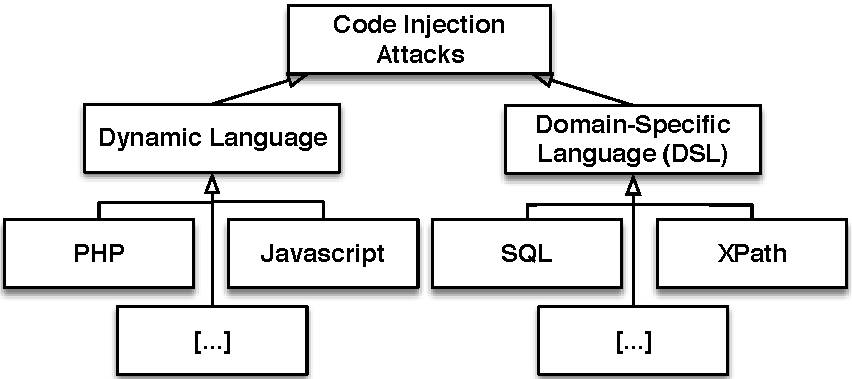
\includegraphics[scale=0.47]{attack-tree-uml.pdf}
\end{center}
\caption{\label{fig:taxonomy}A taxonomy of source
code injection attacks.}
\end{figure}

Code injection attacks can be divided into two categories. The first
involves binary code and the second source code. An
extensive survey on binary code injection attacks can be found
in~\cite{LC03}. Specific advances in exploiting such vulnerabilities
(i.e. ``heap smashing", ``arc injection" and others) have already
been presented~\cite{PB04} and the countermeasures used to detect such
defects have already been surveyed~\cite{YJP12} (many of them are also
included in a book:~\cite{DKZ12} -- Section 13.8). In the present work
we do not include binary code injection, focusing instead on defenses
that protect applications against attacks based on the
source code injection category.

\subsection{Source Code Injection Vulnerabilities}

Figure~\ref{fig:taxonomy} presents a taxonomy of source
code injection attacks. Such attacks may involve source code, either of a
{\it Domain Specific Language} ({\sc dsl}) or a {\it Dynamic Language}.

Application attacks that involve {\sc dsl}s constitute an important
subset of the code injection problem, as {\sc dsl}s like {\sc sql} and
{\sc xml} play an significant role in the development of either web or
mobile applications. For example, many applications have interfaces
where a user enters input to interact with the application's data,
thereby interacting with the underlying Relational Database Management
System ({\sc rdbms}). This input can become part of an {\sc sql} query
and executed on the target {\sc rdbms}. A code injection attack that
exploits the vulnerabilities of these interfaces by taking advantage
of input validation issues like incorrectly passed parameters or
incorrect type handling, is called an {\sc sql} injection
attack~\cite{CERT02,MS09,HVO06,SW06}. By using similar techniques
malicious users can perform other exploits based on {\sc dsl}s,
like {\sc xp}ath~\cite{SW06,CDL07,MKS09}, {\sc xml}~\cite{MSM13}
and No{\sc sql}~\cite{SMS13}. With this kind of attacks,
a malicious user can view sensitive information,
destroy or modify protected data, or even crash the entire
application. {\sc html} is another {\sc dsl} that can be used
for malicious purposes when an application does not properly
handle user supplied data. Based on this vulnerability
an attacker can supply valid {\sc html},
typically via a parameter value, and inject their own
content into the page. {\sc html} injection is mainly associated
with {\sc xss} defects~\cite{HNSHS12}.

A recent class of {\sc cia}s involve dynamic languages like
JavaScript and {\sc php}~\cite{SFVM09,EWKK09,SMS13}. JavaScript
injection attacks, in particular, make up a large subset of dynamic
language-driven attacks. Such attacks are manifested when a web
application accepts and redisplays data of uncertain origin without
appropriate validation and filtering. Based on this flaw, an attacker
can manage to inject a script in the JavaScript engine of a browser
and alter its execution flow~\cite{ELX07}. JavaScript injection
attacks are considered as a critical issue in web application security
mainly because they are associated with major vulnerabilities such as:
{\sc xss} attacks~\cite{SG07}, {\sc csrf} attacks~\cite{BJM08,LZRL09} and
Cross-Channel Scripting ({\sc xcs}) attacks~\cite{W10,BBB09}.
In many cases {\sc xss} attacks involve the injection of
both {\sc html} and JavaScript code.

% {\sc html} injection --- such attacks pose no threat to cookies and session IDs.

\subsection{Exploitation Model}
\label{sec:model}

In this section we provide a step-by-step exploitation model to
understand the process of carrying out application attacks based on
source code injection vulnerabilities.
Figure~\ref{fig:attacks} presents the steps of different application
attacks. For every arrow there is a
corresponding tuple that includes the transition number for
every attack. Every number indicates the number of the
steps taken until we reach this transition.
For the most part, the steps are common in all attacks. This
is because they are based on similar attack vectors as we mentioned in
the previous section. Most importantly,
Figure~\ref{fig:attacks} illustrates in which transitions
the defenses detect corresponding attacks.

A malicious user can initiate the attack through two different routes.
The attacker may use the browser of an innocent user as an attack
vehicle, through which the code will be injected in the application.
For example, the attacker could craft a malicious script into a {\sc url}
and then trick an end user to click on it via social engineering (i.e., phishing ---
{\it transition}: {\sc p-xss} 1.1 \text{\textbar} {\sc n-xss} 1.1 \text{\textbar} {\sc csrf} 1).
Alternatively, the attacker may be able to inject
directly the malicious code in the application. For example, consider
a web application that accepts and redisplays user input
without appropriate validation. An attacker could
upload data containing a specially crafted script (for example, in a
blog comment) to steal the cookies of the visiting users or embed
malicious {\sc sql} code to retrieve all the password entries from a
database ({\it transition}: {\sc dsl} 1 \text{\textbar}
{\sc p-xss} 1 \text{\textbar} {\sc n-xss} 1).
Note that an {\sc xss} attack can start from both routes.

Once the injected code reaches the vulnerable application, it becomes
a part of a value represented by a program variable. The target of the
attack determines the route from now on. In {\sc sql} injection and
{\sc csrf} attacks the injected code becomes part of a query that
finally reaches the database where it is executed. 

{\sc xss} attacks fall ino two categories, {\it non-persistent} and
{\it persistent}. Non-persistent {\sc xss} attacks take place when the
data provided by a user is used immediately by server-side scripts to
parse and display a page of results, without properly sanitizing the
request ({\it transition}: {\sc p-xss} 7 \text{\textbar} {\sc n-xss} 2).
Thus, in a non-persistent {\sc xss} attack the injected code
is never saved on the server and immediately becomes part of the
content that is sent back to a web user.

In persistent {\sc xss} attacks malicious code is saved by the server.
The injected code that is stored on the server-side re-enters the
application's execution flow and becomes part of the content that is
actually sent back afterwards to the user.

\begin{figure*}
\begin{center}
\leavevmode
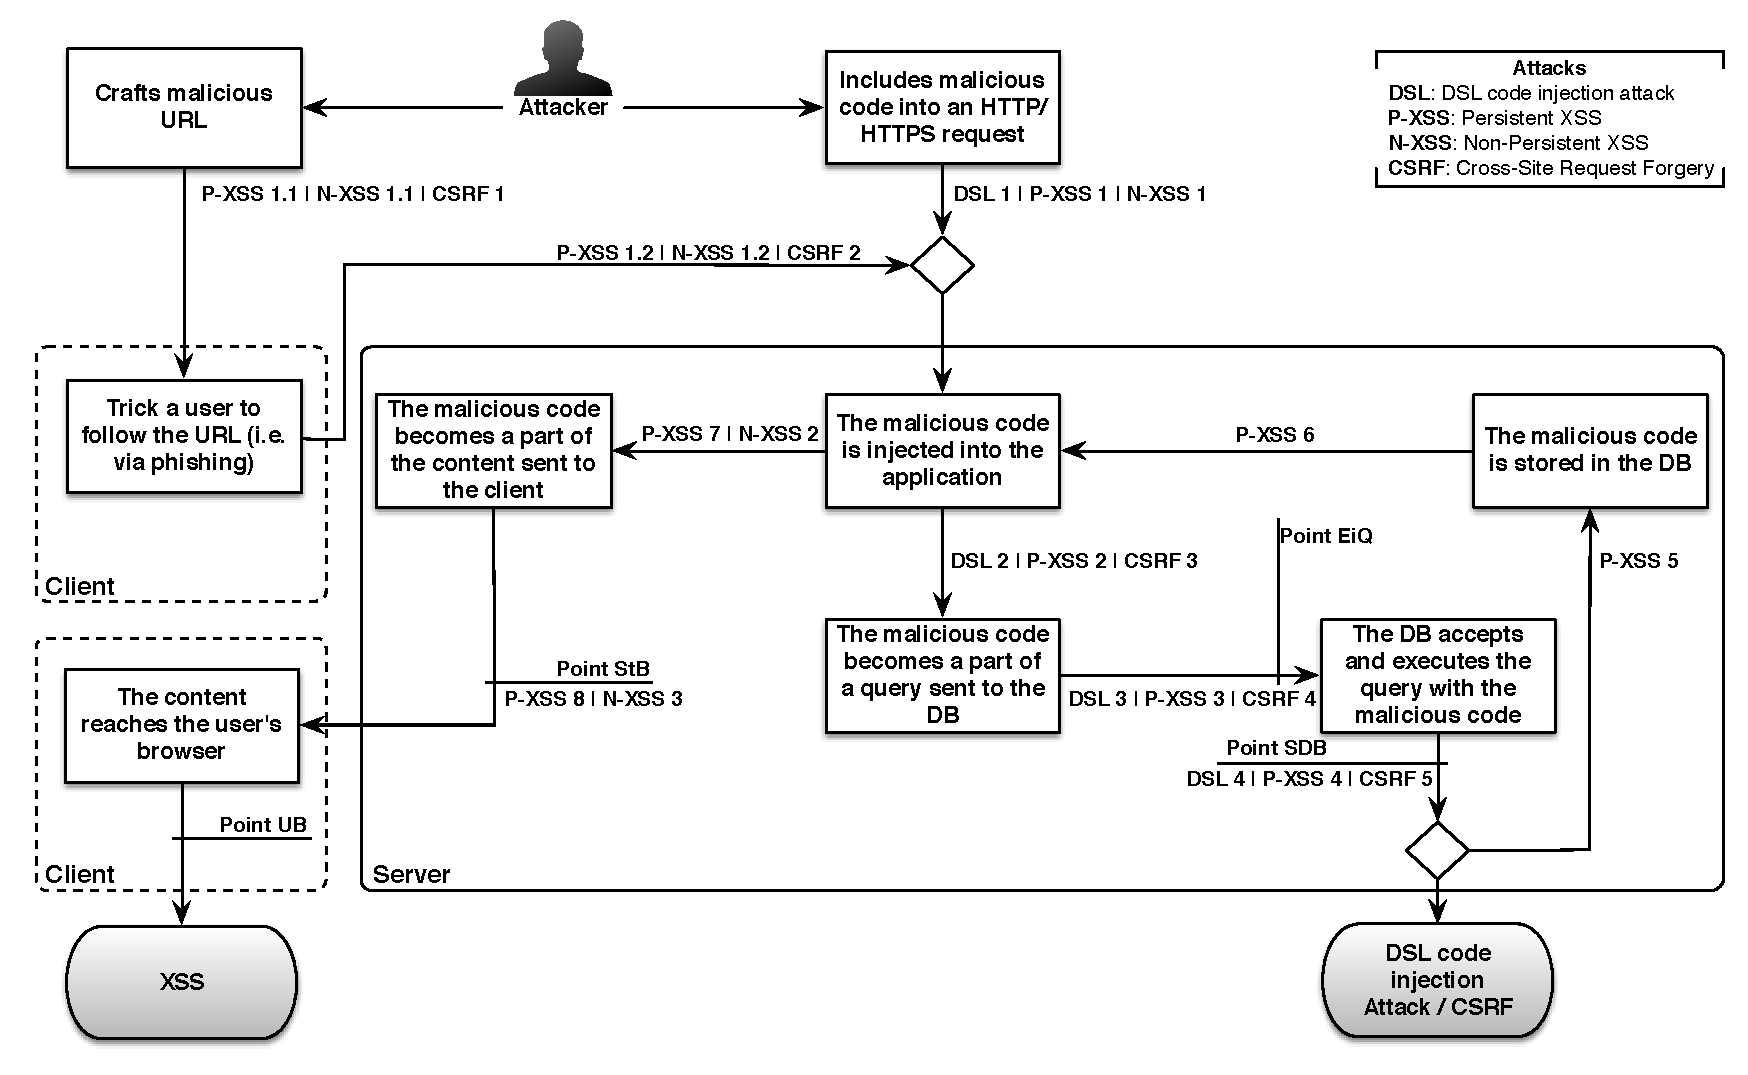
\includegraphics[scale=0.61]{attacks-steps.pdf}
\end{center}
\caption{\label{fig:attacks}Attack model demonstrating web
application attacks based on source
code injection vulnerabilities. For every arrow there is a
corresponding tuple that includes a transition number for
every attack. Every {\it point} indicates a transition where mechanisms
detect attacks. For every point we provide the corresponding
references:
Point {\sc ub}~\cite{KJKV09,TNH07,NSS06,APKLM10,SPPGMMB04,ML10,YCIS07,PSC09,VDDPJ11,OWVS08,DDHPJ10,GC09,VFJKKV07,SLMS14,BV08},
Point {\sc s}t{\sc b}~\cite{RDWDE07,JKK06a,JB07,NLC07,WPLKK09,JEP08},
Point {\sc e}i{\sc q}~\cite{BWS05,SW06,PS11,HCF05,XBS06,PB05,PMP11,MS09,HO05,SMS13},
Point {\sc sdb}~\cite{BK04,LLW02,VMV05}.}
\end{figure*}

\section{Analysis Dimensions}
\label{sec:dimensions}

Research on application attack defense mechanisms has a dual
character. First, a defense mechanism may be important, and therefore
publishable, because it shows that an attack can be detected in a
reliable manner. Secondly, a defense mechanism may be important not
just as a research contribution, but as a practical tool, if it can be
put to use by administrators and users to shield their applications
and services against the detected attacks.

The detection of attacks in a reliable manner can be analyzed using
criteria common with other research fields:
\begin{itemize}
\item Statistical measures that show how reliable the detection really
  is.
\item Research practices that promote replication of the findings.
\end{itemize}

Whether a reliable attack defense mechanism has value in a practical
setting rests on a different set of criteria:
\begin{itemize}
\item What are the overheads imposed by the mechanism?
\item How easy is it to deploy and use the mechanism?
\item How robust is it against ways to circumvent it?
\item At which point of the computation flow does it detect an attack?
\end{itemize}

The first two criteria are \emph{Accuracy} and
\emph{Availability}. The other four criteria are \emph{Computational
  Performance}, \emph{Ease of Use}, \emph{Security}, and
\emph{Point of Detection}.

\subsection{Accuracy}
\label{ssec:diagnostic-performance}

Application attack defense mechanisms
must demonstrate the presence of an attack. This, however, does not
make an application attack defense mechanism immediately useful. A
detection mechanism must be reliable. The accuracy of a detection
mechanism is gauged with the following
metrics~\cite{TDR2013,GFDLS06,A00}:
\begin{itemize}
\item {\bf Sensitivity}, the probability that an attack will be
  caught.
\item {\bf Specificity}, the probability that a normal interaction
  will test negative.
\item {\bf Positive Predictive Value} ({\sc ppv}), the probability that a
  reported attack is a real attack. It is the conditional probability
  that an event is an attack if the detection mechanism flags it as
  such. 
\item {\bf Negative Predictive Value} ({\sc npv}), the probability that if
  nothing is reported no attack has taken place. It is the conditional
  probability that an event is not an attack given that the detection
  mechanism flags it as normal.
\end{itemize}

We will focus on sensitivity and specificity; we will come back to
\textsc{ppv} and \textsc{npv} in Section~\ref{sec:lessons-learned}.
Sensitivity and specifity are defined using the following~\cite{linn2004}:
\begin{itemize}
\item True Positive (\textsc{tp}), an attack that raises an alarm.
\item True Negative (\textsc{tn}), an event that is not an attack and that does
  not raise an alarm.
\item False Positive (\textsc{fp}), an event that although it is not an attack
  raises an alarm.
\item False Negative (\textsc{fn}), an event that although is as attack does
  not raise an alarm.
\end{itemize}

\noindent
With these we can calculate:

\begin{equation}
  \textsc{se} = \textrm{Sensitivity} = \frac{\textsc{tp}}{\textsc{tp}
    + \textsc{fn}}
\label{eq:sensitivity}
\end{equation}

\begin{equation}
  \textsc{sp} = \textrm{Specificity} = \frac{\textsc{tn}}{\textsc{fp}
    + \textsc{tn}}
\label{eq:specificity}
\end{equation}

\noindent
Sensitivity and specificity can be calculated based on test
data alone. To calculate the sensitivity, we run the test on a
controlled environment where we allow only attack events to reach the
system. The ratio of reported attacks over all attacks will give us
the sensitivity. Similarly, to calculate the specificity we can run
the test on a controlled environment where we allow only innocuous
events to reach the system. The ratio of non-reported events over all
events will give us the specificity. 

\subsection{Availability}

To ensure replicability of research results the source code
implementing a detection mechanism should be available to researchers.
Ideally the code should be available under an open source license, so
that it is easy to modify and improve an approach; even when this is
not possible, for whatever reason, it is important to make sure that
all computer code and test data is available noting any restrictions
on accessibility. Availability of computer code has been recognised as
an important issue outside the computer science field: the journal
Nature, in a recent editorial, adopted a publication policy stressing
access to code and data~\cite{nature2014}. At a time and date that the
merits of open access to code are discussed in non computer science
journals~\cite{easterbrook2014} we should expect computer scientists
to lead the way.
 
\subsection{Computational Performance}

All detection mechanisms extract a cost for their use, as they
introduce some amount of extra computation on an existing application.
The extra computation depends on the exact defense mechanism. For
example, it may be some form of run-time checking, or some form of
obfuscation. Also depending on the mechanism, the cost may be incurred
on different places: it may take place on a server, affecting service
performance, or it may take place on the client, or both. The
usefulness of a detection mechanism depends therefore on the
computational cost it requires and on where it extracts it, as
different overheads may be acceptable server-side than client-side.
For example, reporting absolute measurements gives little information
on the real overhead, unless separate measurements are given for the
system under study with and without the proposed mechanism. Percentage
measurements are normally better. Outliers may be important. It is
always necessary to describe the experimental setup.

Performance evaluation rests on strong foundations~\cite{jain1991} and
is a vibrant field as new technologies emerge~\cite{gregg2014}.
Although it may not be necessary to conduct a comprehensive
performance evaluation analysis for a defense mechanism, the more
performance evaluation is provided for a mechanism the more valuable
it becomes as a practical approach.

\subsection{Ease of Use}
\label{sec:deployment}

The value of a detection mechanism as a practical tool depends on how
it is to deploy it in a production setting. That is independent of the
value of a detection mechanism as a research finding. Devising a
mechanism to detect a hitherto undetectable class of attacks may be an
excellent research contribution that merits publication; it may also
be heavily cited and open the road to other, practical
implementations in the future. 

The ease of use, in turn, depends on several factors. The detection
mechanism may be deployed server-side or client-side, or both.
Deployments on just the server or the client are easier to handle than
deployments on both of them. The mechanism may be an add-on, or
plugin, on existing software, client or server, or it may be tightly
integrated with existing software, requiring rebuilding from source
code. 

No matter where it gets installed, the means of installation influences
ease of use. A detection mechanism that comes with ready to install
packages will trump a detection mechanism that only exists in the form
of source code. 

\subsection{Security}

Defenders and attackers are often caught in a cat-and-mouse game,
where countermeasures are bypassed by canny attacks, which are caught
by more sophisticated countermeasures, yet again bypassed by cannier
attacks, and so on. We use Security to refer to the ability of a
detection mechanism to resist being circumvented. 

A mechanism that has not been bypassed is not eternally secure, as it
is possible that a bypass method will be discovered in the future. We
examine the various approaches on the knowledge we have to this date,
that is, whether there are known ways to bypass the detection
mechanism today.

\subsection{Point of Detection}

Detection mechanisms vary on the location where they detect an attack.
There are four different points where an attack can be caught, as seen
in Figure~\ref{fig:attacks}:
\begin{itemize}
\item At the user's browser (Point {\sc ub}).
\item En route from the server to the user's browser --- in most cases
within a proxy (Point {\sc s}t{\sc b}).
\item Embedded in a query, but before it reaches the server's database
  (Point {\sc e}i{\sc q}).
\item After the malicious code has been executed on the server's
  database (Point {\sc sdb}).
\end{itemize}

\section{Defenses}
\label{sec:defs}

\begin{figure*} [ht]
\begin{center}
\leavevmode
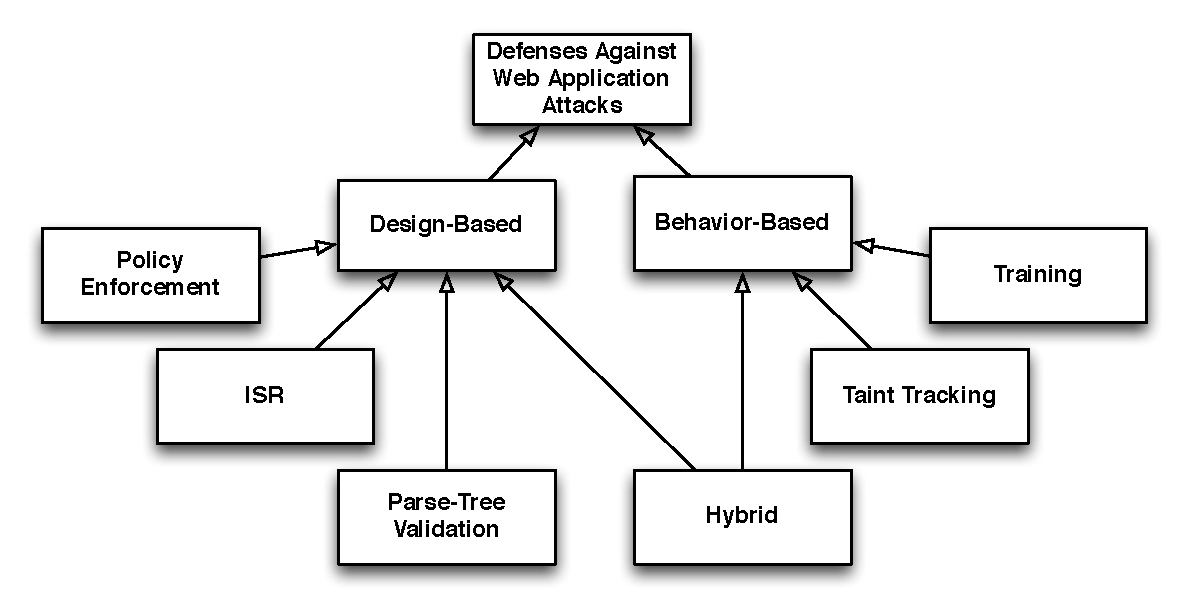
\includegraphics[scale=0.65]{defenses.pdf}
\end{center}
\caption{\label{fig:defenses}The basic categories of countermeasures
against web application attacks, based on source code
injectiion. For each approach we provide the references
that present corresponding mechanisms:
{\bf 1}~\cite{NSS06,JKK06a,KKVJ06,KJKV09,TNH07,RDWDE07,YCIS07,OWVS08,PSC09,ML10,DDHPJ10,PS11,VDDPJ11,BV08,LV09},
{\bf 2}~\cite{BK04,JB07,GC09,APKLM10},
{\bf 3}~\cite{BWS05,SW06},
{\bf 4}~\cite{HCF05,PB05,XBS06,NLC07,VFJKKV07,PMP11,SLMS14},
{\bf 5}~\cite{LLW02,HO05,HO06,HO05b,VMV05,JEP08,WPLKK09,MS09,MKS09,MKLS11},
{\bf 6}~\cite{BV08,LV09,SMS13}.}
\end{figure*}

We categorize and describe the various mechanisms developed to detect
the attacks described in Section~\ref{sec:attacks} on the dimensions
we proposed apart from availability, which we treat separately in the
``Discussion" section (\ref{sec:discussion}).

Figure~\ref{fig:defenses} presents a taxonomy of the
defenses that protect web applications against attacks based on
code injection vulnerabilities.
We can identify three approaches:
{\it etiological}, {\it symptomatic} and {\it hybrid}.
The etiological category involves mechanisms designed to
stop attacks based on their causes and origins~\cite{JL75,L81}. 
The symptomatic category incorporates a variety of schemes that
inspect the behavior of applications and detect attacks based on
their undesirable symptoms~\cite{D76,A00}.
Hybrid mechanisms borrow characteristics from both
categories. Table~\ref{tab:comp} groups the various subcategories and
for every mechanism provides the following:

\begin{enumerate}
\item The number of times the corresponding publication has been cited.
\item Accuracy and computational overhead measurements.
\item The attacks that the mechanism detects.
\end{enumerate}

Finally, as we mentioned in Subsection~\ref{sec:model},
Figure~\ref{fig:attacks} illustrates for each mechanism (found in the
figure's caption), the point where it detects attacks.

\subsection{Etiological}
\label{sec:prot}

There exist three basic etiological approaches used to protect web
applications from source code injection attacks.

\subsubsection{Parse-Tree Validation}
\label{sec:tree}

The key idea behind this approach is to compare
the tree representation of the abstract syntactic
structure of the source code that is about to be
executed with the one that was originally intended.
If the trees diverge, the application is probably
under attack.

In the case of {\sc dsl} injection attacks, mechanisms check 
the query before the inclusion of user input with the one
resulting after the inclusion of user input.
Both mechanisms that implement this approach,
{\sc sqlg}uard~\cite{BWS05} and
{\sc sql}check~\cite{SW06} are pretty similar
and detect the attack before a query reaches the
database (Point {\sc e}i{\sc q}).
Contrary to {\sc sqlg}uard (and other
mechanisms as we will observe), {\sc sql}check has been
extensively tested in terms of accuracy
as it can be seen in Table~\ref{tab:comp}.
A disadvantage of those mechanisms is that the
application must be modified in every code fragment
that sends an {\sc sql} query to the database for execution.

Parse-tree validation seems to be an efficient approach
to detect {\sc dsl} code injection attack,
especially in the case of the {\sc sql}check
implementation. This however does not apply in
the case of the mechanisms that borrow elements from
this approach and examine the syntax trees
of scripts to detect JavaScript-driven {\sc xss} attacks
as we will see in Subsection~\ref{sec:hybrid}.

\subsubsection{Policy Enforcement}
\label{sec:policy}

This approach is used to detect {\sc xss} and {\sc csrf} attacks.
When using a framework that implements
this approach, developers must define
specific security policies on the server side.
Policies can be expressed through JavaScript extensions,
pattern matching or syntax specific settings.
Then the policies are enforced either in the user's
browser at runtime or in a server-side proxy that intercepts
server responses.

{\it Noxes}~\cite{KKVJ06,KJKV09} is the only
framework that partially allows the web
user to specify policies to prevent {\sc xss} attacks.
The key idea behind Noxes is to parse
the {\sc html} that reaches the browser to
find static {\sc url} references. Then, based on
a set of policies Noxes allows or blocks
the request (Point {\sc ub}). Such policies
can be also provided by the server (i.e. ``never
follow a link that leads to the malicious.com
web site"). The main issue with Noxes is that
it does not deal with JavaScript-driven {\sc xss}
attacks which is currently the most popular
{\sc xss} attack vector.

A number of the frameworks define policies
based on information and features provided by
the Document Object Model ({\sc dom}) of a web page.
Specifically, developers must place all legitimate
scripts inside {\sc html} elements like {\tt div}.
The web browser (Point {\sc ub}), parses the
{\sc dom} tree and executes scripts only when they
are contained in such elements. All other scripts
are treated according to the policies defined
on the server. Frameworks that support this
functionality are {\sc beep}~\cite{TNH07}
and {\sc dsi}~\cite{NSS06}. The main problem with
the above mechanisms is that they are vulnerable
to non-persistent {\sc xss} attacks that alter
the {\sc dom} of an already rendered
page~\cite{APKLM10}.
In addition, a recent variation of JavaScript
injection attacks known as return-to-JavaScript
attack can be used to bypass the above mechanisms
as described extensively in reference~\cite{APKLM10}.
% Such attacks share
% many similarities with the {\it return-to-lib}
% attack~\cite{SPPGMMB04}. 
%% PL Explain what it does, I guess it's what you go on to say
%% directly below?
% When performing an attack like this the malicious user transfers the
% execution to points that contain script code which in turn is used to
% perform the attack.

Another policy enforcement approach introduces
policies directly either in {\sc html} or JavaScript code
to confine their behavior. {\it BrowserShield}~\cite{RDWDE07}
acts as a proxy on the server side (Point {\sc s}t{\sc b}) to
parse the {\sc html} of server responses and identifies
scripts. Then, it rewrites them into safe equivalents
and protects the web user from exploits
that are based on reported browser vulnerabilities.
{\it ConScript}~\cite{ML10}, {\it CoreScript}~\cite{YCIS07}
and the framework by {\it Phung et al.}~\cite{PSC09}
extend JavaScript with new primitive functions that
provide safe methods to protect potentially vulnerable
JavaScript functions. In both cases, policy enforcement takes
place on the JavaScript engine of the browser (Point {\sc ub}).
In this way, {\sc xxs} attacks that take advantage
functions like {\tt write} and {\tt eval}, which are
used to assemble innocuous-looking parts into harmful
strings,\footnote{The infamous Sammy worm that
infected MySpace in 2005~\cite{SP07,ELX07}
utilized the {\tt eval} function to assemble a
script with malicious behavior.} would fail.

An issue regarding the above frameworks
involves features like script inclusion
and {\tt iframe} tags. Even though they allow developers
decide if they will disable them or not,
this is unpractical because such features are quite popular.
If developers choose to use them, these frameworks cannot
define policies that restrict the behavior of third-party
scripts introduced by such features. For instance,
consider a web page (foo.net) that prints the value
of a query parameter ({\tt query}) from the
page's {\sc url} in the web page's content
without escaping the value. A malicious user
can take advantage of this and inject an {\tt iframe}
into the page to steal the user's cookie and
send it via an image request to a web site
that he or she controls (malicious.com).
This could be achieved by including the following
link to the malicious web site (or send it via phishing
email) and induce the user to click on it:

\lstset{language=VBScript, basicstyle=\footnotesize\ttfamily,}
\begin{lstlisting}
http://foo.net/vulnerable.html?query=
<iframe src="javascript:document.body.innerHTML=+
'<img src=\"http://malicious.com/?c=
'+encodeURIComponent(document.cookie)+'\">'">
</iframe>
\end{lstlisting}

\noindent
{\it WebJail}~\cite{VDDPJ11}, and
{\sc soma}~\cite{OWVS08} are two frameworks that
can actually detect such an attack (Point {\sc ub}).
To achieve this, {\sc soma} requires site administrators
to specify legitimate, external domains for sending
or receiving information in order to approve interactions
between them and the protected web site. As a result,
{\sc soma} can also detect {\sc csrf} attacks.
WebJail, contains the functionality of
third-party scripts by introducing a web component
integrator that restricts the access that these scripts
may have to either the data or the functionality of other components

Policy enforcement mechanisms that detect {\sc csrf}
attacks are usually implemented in the form of a
server-side proxy (Point {\sc s}t{\sc b})
interposing on the client-server communication, and modifying
it. {\it NoForge}~\cite{JKK06a}
parses the {\sc html} server responses
and adds a token to every {\sc url} referring to this
server. Then it associates the token with the cookie
representing the session {\sc id} for the application.
When a request is received, the mechanism checks
if the request contains the token related
to the session {\sc id}. A disadvantage of NoForge
is that {\sc html} that is dynamically created within
the browser will not include the token.
Thus, sites that create their {\sc html} on the client
will remain vulnerable. In addition, it does not
support cross-origin requests.
{\it j{\sc csrf}}~\cite{PS11}
has a very similar functionality and meanwhile
addresses the above problems.
Finally, {\it CsFire}~\cite{DDHPJ10}
examines cross-domain interactions, to design a
cross-domain policy on the client's side (Point {\sc ub}).
The policy is based on the concept of a relaxed
same-origin policy that allows communication between
sub-domains of the same registered domain.

Most of the aforementioned frameworks involve
several deployment issues since they
require significant source modifications by the
developers on the server-side in order to
introduce the policies.

\subsubsection{Instruction Set Randomization (ISR)}

{\sc isr} is a method that has been applied to counter different kinds
of application attacks~\cite{K09b,KKP03}. The main idea behind it is
to separate code from data by randomizing the legitimate code's
execution environment. In this way, the malicious code injected by the
attackers who do not know the randomization algorithm, will not get
executed.

{\it {\sc sql}rand}~\cite{BK04} implements {\sc isr} to detect {\sc
  sql} injection attacks. It allows programmers to create {\sc sql}
statements using randomized instructions instead of standard keywords.
The modified queries are reconstructed at runtime using the same key
that is inaccessible to the malicious user. {\sc sql}rand is one of
the few mechanisms that detect {\sc sql} injection attacks on the
database level (Point {\sc sdb}).

In the case of {\sc xss} attacks that are based on JavaScript or {\sc
  html}, consider a {\sc xor} function that encodes all source of a
web page on the server-side and then, on the client-side, the web
browser decodes the source by applying the same function again (Point
{\sc ub}). Variations of this approach include {\it
  Noncespaces}~\cite{GC09} and {\it x{\sc js}}~\cite{APKLM10}, which
randomize the instruction set of {\sc html} and JavaScript
respectively. Contrary to x{\sc js}, in Noncespaces administrators
must set specific policies in a manner similar to a firewall
configuration language. This fact, together with the insufficient
testing of the mechanism (see Table~\ref{tab:comp}) brings up
questions concerning its accuracy. {\it {\sc
    sm}ask}~\cite{JB07} is another framework that was inspired by {\sc
  isr}. To detect {\sc xss} attacks it searches for {\sc html} and
JavaScript keywords within the application's legitimate code. This is
done before the processing of an {\sc http} request. When it finds one
it adds a token to it. This results to a ``code mask". Then, before
sending the resulting {\sc html} data to the web user, the framework
searches the data for illegal code by using the same keywords (Point
{\sc s}t{\sc b}). Since all legitimate code has been ``masked", the injected
code can be identified. The pre- and post-processing of the code
though, may add a significant overhead to the application.
Unfortunately, the authors of {\sc sm}ask did not provide measurements
regarding the computational performance of the tool (see
Table~\ref{tab:comp}).

{\sc isr} is a deterministic approach that can be applied to detect
different attacks in an efficient manner. However, Sovarel et
al.~\cite{SEP05} have investigated thoroughly the effectiveness of
{\sc isr} and showed that a malicious user may be able to circumvent
it by determining the randomization key and their results indicate
that doing {\sc isr} in a way that provides a certain degree of
security against a motivated attacker is more difficult than
previously thought. Furthermore, developers who wish to use such
mechanisms must follow good coding practices and never show a
randomized code statement in any case (i.e. an exception error)
because in this way they will reveal the encoding key.

Even though the above implementations impose a low computational
overhead, they impose an infrastructure overhead. In particular, in
{\sc sql}rand requires the integration of a proxy within the database
server, while Noncespaces and x{\sc js} require modifications on both
the server and the client.

\subsection{Symptomatic}

In this section we examine the two main symptomatic
approaches.

\subsubsection{Taint Tracking}
\label{sec:taint}

A taint tracking scheme marks untrusted
(``tainted") data (for instance, a variable set
by a field in a web form) and traces its flow through
the program. If the variable is used in an expression
that sets another variable, that variable is also
marked as untrusted and so on. If any of these variables
is used to execute a potentially risky command (``sink") the
scheme may act accordingly.

Taint tracking is provided as a feature in some programming languages,
such as Perl and Ruby. By enabling the feature, Perl would refuse to
run code vulnerable to an {\sc sql} injection attack (consider a
tainted variable being used in a query) and would exit with an error
message.

There are different implementations of this approach
in terms of how the tainted data is marked and observed,
and how attacks are detected.
For example, {\it Haldar et al.}~\cite{HCF05} have implemented
their scheme for the Java Virtual Machine ({\sc jvm})
where they instrument various classes. When a
tainted string is used as an argument to a sink method
then an exception is raised (Point {\sc e}i{\sc q}).

It is possible to apply further checks when it is established that
tainted data have reached a sink (Point {\sc e}i{\sc q}). {\it Xu et
  al.}~\cite{XBS06} track taint information at the level of bytes in
memory. To distinguish between legitimate and malicious uses of
untrusted data that reach a sink, they search the data for suspicious
symbols by using regular expressions. {\sc csse}~\cite{PB05}
associates tainted data with specific metadata. Such metadata include
the origins of tainted data, its propagation within the application,
and others. When tainted data reaches a sink, {\sc csse} performs
syntactic checks based on the aforementioned metadata (Point {\sc e}i{\sc q}).
{\it {\sc php} Aspis}~\cite{PMP11} works in a similar way. To obtain
metadata, it takes advantage of {\sc php} arrays data structure.
Finally, {\sc wasc}~\cite{NLC07} analyzes {\sc html} responses to check
if there are tainted data that contain scripts (Point {\sc s}t{\sc b}).

A recent study~\cite{NBR14} showed that there are ways to circumvent
the majority of the above schemes. Furthermore, most of them are not
easy to deploy since the majority of input vectors, string operations
and output vectors of the application must be instrumented.

{\it Vogt et al.}~\cite{VFJKKV07} have developed a tainting scheme
that follows a different approach. Contrary to the aforementioned
schemes that operate on the server side, they track sensitive
information on the client side (Point {\sc ub}). This is a form of
positive taint tracking, where taint data is considered to be
legitimate. Their scheme detects JavaScript-driven {\sc xss} attacks
by ensuring that a script can send sensitive user data only to the
site from which it came from.
{\it Stock et al.}~\cite{SLMS14} propose a scheme that also operates
in the browser (Point {\sc ub}). The scheme focuses on the detection of
{\sc dom}-based {\sc xss} attacks. In such an attack, the malicious
payload is executed as a result of the modification of the {\sc dom}
environment so that the client-side code runs in an unanticipated
manner even if the {\sc http} response that triggers the injection
seems legitimate. The scheme is different from the previous one
because it marks and observes data that are considered harmful.
Specifically, it employs a taint-enhanced JavaScript engine that
tracks the flow of attacker-controlled data. To detect potential
attacks the scheme utilizes {\sc html} and JavaScript parsers that can
identify the generation of code coming from tainted data.

\subsubsection{Training}
\label{sec:train}

Training techniques are based on the ideas of Denning's original
intrusion detection framework~\cite{Den87}. In particular, a training
mechanism registers all valid legitimate code statements during a
training phase (mostly in the form of signatures). This can
be done in various ways according to the implementation. Then, only
those will be recognized and approved for execution
during production.

Training methods that detect {\sc dsl}-driven injection attacks
generate and store valid code statements (i.e. {\sc sql} or {\sc
  xp}ath queries) in various forms, and detect attacks as outliers
from the set of valid code statements. An early approach, {\it {\sc
    didafit}}~\cite{LLW02} detects {\sc sql} injection (Point
sdb) attacks by recording all database transactions
(stripped from user input). Subsequent
refinements by Valeur et al.~\cite{VMV05} tagged each transaction with
the corresponding application as an extension of their anomaly
detection framework called {\it libAnomaly}. {\it {\sc
    sd}river}~\cite{MS09,MKS09,MKLS11} is a signature-based mechanism
that prevents {\sc sql} and {\sc xp}ath injection attacks. The
signatures generated during a training phase are based on features
that can depend either on the code statement or on its execution
environment (i.e. the stack trace). Then, at runtime, the mechanism
checks all statements for compliance and can block code statements
containing injected elements (Point {\sc e}i{\sc q}). {\sc
  amnesia}~\cite{HO05,HO06,HO05b} is a tool that also detects {\sc
  sql} injection attacks (Point {\sc e}i{\sc q}) by associating a query model
with the location of every {\sc sql} statement within the application.
Then, at runtime, it monitors the application's execution to detect
when {\sc sql} statements diverge from the expected model.

Various countermeasures against {\sc xss} attacks follow a similar
pattern. {\it {\sc swap}}~\cite{WPLKK09} creates a unique identifier
({\it script {\sc id}}) for every legitimate script on the server.
Then, a JavaScript detection component placed in a web proxy (Point
{\sc s}t{\sc b}) searches for injected scripts with no corresponding {\sc id}
in the server's responses. If no injected scripts are found, the proxy
forwards the request to the client. This mechanism is relatively
inflexible since it does not support dynamic scripts. In addition it
imposes a significant overhead (see Table~\ref{tab:comp}). The authors
of {\it {\sc xssds}}~\cite{JEP08} have implemented a similar mechanism
that also supports dynamic and external scripts. Specifically, during
training phase they build a list of all benign scripts. In the case of
external scripts they keep a white list of all the valid domain names
that contain scripts used by the application.

Defenses based on training include some mechanisms that can be easily
circumvented. For example, {\sc didafit} and {\it libAnomaly}
do not tag transactions with their corresponding call-sites.
In this case a false negative result
is prominent. For instance, consider an application that will send the
password for a forgetful user via email by executing the following
query:
\bgroup
\lstset{language=SQL}
\begin{small}
\begin{lstlisting}
SELECT password from userdata WHERE id = 'Alice'
\end{lstlisting}
\end{small}
\egroup
\noindent
This same application could allow users to lock their terminal,
but allow the unlocking either with the user's password or with
the administrator password (the 4.3 {\sc bsd} {\em lock} command
behaved in this peculiar way).
The corresponding query to verify the password on the locked
workstation would be as follows:
\bgroup
\lstset{language=SQL}
\begin{small}
\begin{lstlisting}
SELECT password from userdata WHERE id = 'Alice' OR
id = 'admin'
\end{lstlisting}
\end{small}
\egroup
\noindent
In this case {\sc didafit} and {\it libAnomaly}, could be easily escaped
since a malicious user, could obtain the administrator's password
by email by entering on the password retrieval form
as his user identifier the following:
\bgroup
\lstset{language=SQL}
\begin{small}
\begin{lstlisting}
nosuchuser' OR id = 'admin
\end{lstlisting}
\end{small}
\egroup
\noindent

However, mechanisms that create signatures that involve
elements not only associated with the code statements
(i.e. {\sc amnesia} and {\sc sd}river)
could detect such attacks. Specifically,
{\sc sd}river associates a complete stack trace with the
root of an {\sc sql} statement, thus it can correlate
queries with their call sites and detect attacks
like the aforementioned one.
Furthermore, training tools that detect
{\sc xss} attacks based on JavaScript injection
would fail to detect a return-to-JavaScript
attack~\cite{APKLM10}.

In general, the detection accuracy of training approaches is
heavily based on the coverage that is achieved during the
training phase. If the coverage is insufficient the
production of false alarms is very likely.
In addition, when a code statement is altered, a new
training phase is necessary.

Most of the mechanisms above are relatively easy to deploy.
{\sc dsl} injection attack countermeasures
can be retrofitted to a system typically by changing
some configuration files (i.e. {\sc sd}river). This does not apply
to {\sc amnesia} though, since significant source code
modifications are required for every query that exists
in the application. Finally, {\sc swap} and {\sc xssds}
are implemented within a proxy on the server-side.

\subsection{Hybrid}
\label{sec:hybrid}

This category includes mechanisms that borrow
characteristics from more than one of the above categories.
Two of them focus on the detection of {\sc xss}
attacks and one of them focuses on {\sc dsl} code
injection attacks.

{\sc xss-guard}~\cite{BV08} is a training scheme that also employs
parse-tree validation. During training, the scheme maps legitimate
scripts to {\sc http} responses. During production {\sc xss-guard}
retrieves for every script included in a response its parsed tree and
checks if it is one of those previously mapped to this response. Apart
from the comparison of the parsed trees, {\sc xss-guard} checks also
for an exact match of lexical entities. To achieve this, the scheme
utilizes that data structures of Firefox's JavaScript engine (Point
{\sc ub}). However, string literals are not compared literally and
therefore a false negative result could occur if an adversary performs
a mimicry attack~\cite{WS02}. For example, consider a banner rotator
that every time it runs, it creates a value that depends on the
current date and the length of the array that contains the references
of the various images to be displayed. Then, based on this value it
shows a specific image to a user. In a vulnerable web site that allows
users to post data and contains this banner rotator, a malicious user
could create and store a script that has the same code structure, with
the same JavaScript keywords contained in the rotator script.
%% PL You mean like the rotator?
In this script the attacker could also include references to tiny
images hosted on a web server that is maintained by him in order to
retrieve the {\sc ip} addresses of the users that visit the vulnerable
site.

{\it Blueprint}~\cite{LV09} is a policy enforcement framework that
also utilizes parsed trees to detect {\sc xss} attacks. To guarantee
that untrusted content is not executed, Blueprint generates on the
server-side a parsed tree from untrusted {\sc html} to ensure that it
does not contain any dynamic content. Then the parsed tree is
transfered to the document generator of the browser (Point {\sc ub})
where untrusted browser parsing behavior is ruled out. Blueprint is an
efficient countermeasure but it imposes a significant overhead due to
its extensive parsing (see Table~\ref{tab:comp}).

{\it Diglossia}~\cite{SMS13} combines positive taint tracking (see
Subsubsection~\ref{sec:taint}) together with parse-tree validation.
Diglossia was based on the theory of Ray and Ligatti~\cite{RL12b}
(also see Section~\ref{sec:attacks}) to detect {\sc dsl} code
injection attacks. In addition, it is actually the first, and so far
the only framework that detects No{\sc sql} injection attacks. When an
application computes an output string (query), Diglossia computes a
``shadow" of this string. Specifically, it maps all characters
introduced by the application to a shadow character set. This set does
not contain any characters coming from the tainted input. Then, the
scheme creates the tree of the query that is about to be executed and
compares it with the parsed tree of the ``shadow" (Point {\sc e}i{\sc q}). If
the trees are not equal the application is probably under attack. Note
that Diglossia can be bypassed in the same way as other taint
tracking approaches as described in reference~\cite{NBR14}.
%% PL which way is this exactly?

\begin{landscape}
\begin{table}
    \caption{Comparison summary of mechanisms developed to counter application attacks based on source code injection.}
    \label{tab:comp}
\centering
    \begin{threeparttable}
    \begin{small}
\scalebox{0.99}{
    \begin{tabular}{l|c|c|cc|c}
    \thickhline
    \bf{Approach}
	& \bf{Mechanism}
	& \bf{\# of Citations}
  & \multicolumn{2}{|c|}{Requirements\tnote{1}}
	& \bf{Attack} \\
	&&& \bf{TP,TN,FP,FN}\tnote{2}
	& \bf{Computational Overhead}\tnote{3} & \\
    \thickhline
  \multirow{2}{*}{Parse-Tree Validation}
  &   {\it {\sc sqlg}uard}~\cite{BWS05} & 243 & ({\sc na},{\sc na},{\sc na},{\sc na})\_{\bf ?} & 3\% ({\sc s}) & {\sc sql} injection \\
  &   {\it {\sc sqlc}heck}~\cite{SW06} & 402 & (36848,7648,0,0)\_r & 3ms per query ({\sc s}) & {\sc sql} injection \\
  \hline
  \multirow{12}{*}{Policy Enforcement}
  &   {\it {\sc dsi}}~\cite{NSS06} & 135 & (5268,{\sc nq},46,15)\_r & 1.85\% ({\sc c}) & {\sc xss} \\ 
  &   {\it NoForge}~\cite{JKK06a} & 35 & (7,{\sc nq},{\sc nq},0)\_r & {\sc na} ({\sc s}) & {\sc csrf} \\
  &   {\it Noxes}~\cite{KKVJ06,KJKV09} & 268,40 & (3,{\sc na},{\sc na},0)\_r & {\sc na} ({\sc c}) & {\sc xss} \\
  % &   {\it {\sc met}}~\cite{ELX07} & 58 & ({\sc na},{\sc na},{\sc na},{\sc na})\_{\bf ?} & {\sc na} & {\sc xss} \\ 
  &   {\it {\sc beep}}~\cite{TNH07} & 282 & (61,{\sc na},{\sc na},0)\_r & 14.4\% ({\sc c}) & {\sc xss} \\
  &   {\it BrowserShield}~\cite{RDWDE07} & 219 & (19,{\sc nq},0,0,)\_r & 8\% ({\sc s}) & {\sc xss} \\ 
  &   {\it CoreScript}~\cite{YCIS07} & 181 & ({\sc nq},{\sc nq},{\sc nq},{\sc na})\_s & {\sc nq} ({\sc c}) & {\sc xss} \\
  &   {\it {\sc soma}}~\cite{OWVS08} & 46 & (5,{\sc na},{\sc na},0)\_s & 5.58\% ({\sc c}) & {\sc xss}, {\sc csrf} \\
  % &   {\it Barth et al.}~\cite{BJM08} & 271 & & {\bf ?} & {\sc csrf} \\
  &   {\it Phung et al.}~\cite{PSC09} & 75 & (37,{\sc na},{\sc na},4)\_r & 5.37\% ({\sc c}) & {\sc xss} \\
  &   {\it ConScript}~\cite{ML10} & 122 & ({\sc na},{\sc na},{\sc na},{\sc na})\_{\bf ?} & 7\% ({\sc c}) & {\sc xss} \\
  &   {\it CsFire}~\cite{DDHPJ10} & 35 & (419582,1141807,0,3)\_r\tnote{4} & {\sc na} ({\sc c}) & {\sc csrf} \\
  &   {\it j{\sc csrf}}~\cite{PS11} & 2 & (2,{\sc na},{\sc na},0)\_r & 2ms ({\sc s}) & {\sc csrf} \\
  &   {\it WebJail}~\cite{VDDPJ11} & 25 & ({\sc na},{\sc na},{\sc na},{\sc na})\_{\bf ?} & $\sim$7ms ({\sc c}) & {\sc xss} \\
  % &   {\it TreeHouse}~\cite{IW12} & 18 & ({\sc na},{\sc na},{\sc na},{\sc na})\_{\bf ?} & 757–-1218ms & {\sc xss} \\
  % &   {\it {\sc js}and}~\cite{AVBPDP12} & 22 & ({\sc na},{\sc na},{\sc na},{\sc na})\_{\bf ?} & up to 31.2\% & {\sc xss}\\
  % \hline
  % \hline 
  % \multirow{3}{*}{Securing Mashups}
  % &   {\it {\sc om}ash}~\cite{CHC08} & 58 & ({\sc na},{\sc na},{\sc na},{\sc na})\_{\bf ?} & {\sc nq} & {\sc csrf} \\
  % &   {\it Mashup{\sc os}}~\cite{WFHJ07} & 149 & ({\sc na},{\sc na},{\sc na},{\sc na})\_{\bf ?} & 1--59\% & {\sc xss} \\
  \hline
  \multirow{4}{*}{{\sc isr}}
  &   {\it {\sc sql}rand}~\cite{BK04} & 286 & (3,{\sc na},{\sc na},0)\_a & $\le$6.5{\it ms} ({\sc s}) & {\sc sql} injection \\
  &   {\it {\sc sm}ask}~\cite{JB07} & 27 & (5,{\sc nq},{\sc nq},{\sc nq})\_r  & {\sc na} ({\sc s}) & {\sc sql} injection, {\sc xss} \\
  &   {\it Noncespaces}~\cite{GC09} & 109 & ({\sc nq},{\sc na},{\sc na},0)\_r &  10.3\% ({\sc c}) & {\sc xss} \\ 
  &   {\it x{\sc js}}~\cite{APKLM10} & 18 & (1380,{\sc na},{\sc na},1)\_r & 1.6--40{\it ms} ({\sc c}) & {\sc xss} \\
  \thickhline
  \thickhline
	\multirow{7}{*}{Taint Tracking}
  &   {\it Haldar et al.}~\cite{HCF05} & 177 & (2,{\sc na},{\sc na},0)\_s & {\sc nq} ({\sc s}) & {\sc sql} injection, {\sc xss} \\ 
	&  	{\sc csse}~\cite{PB05} & 312 & (7,{\sc nq},{\sc nq},{\sc nq})\_r & 2--10\% ({\sc s}) & {\sc sql} injection, {\sc xp}ath, {\sc xss} \\
	% &  	{\it SecuriFly}~\cite{MLL05} & 31 & \xmark,\tick & 9--125\% & {\sc sql} injection, {\sc xss} \\ 
	&  	{\it Xu et al.}~\cite{XBS06} & 297 & (9,{\sc nq},0,{\sc nq})\_r & average 76\% ({\sc s}) & {\sc sql} injection, {\sc xss} \\ 
  &  	{\it {\sc wasc}}~\cite{NLC07} & 31 & ({\sc nq},{\sc nq},{\sc nq},{\sc nq})\_r & up to 30\% ({\sc s}) & {\sc sql} injection, {\sc xss} \\
	&  	{\it Vogt et al.}~\cite{VFJKKV07} & 322 & ({\sc nq},{\sc nq},{\sc nq},{\sc na})\_r & {\sc nq} ({\sc s}) & {\sc xss} \\
	&  	{\it {\sc php} Aspis}~\cite{PMP11} & 12 & (12,{\sc nq},{\sc nq},2)\_r & 2.2$\times$ ({\sc s}) & {\sc sql} and {\sc php} injection, {\sc xss} \\
	& 	{\it Stock et al.}~\cite{SLMS14} & 0 & (1169,{\sc na},{\sc na},0)\_r & 7--17\% ({\sc c}) & {\sc dom}-based {\sc xss} \\
	\hline 
  \multirow{6}{*}{Training}
  &   {\it {\sc didafit}}~\cite{LLW02} & 85 & ({\sc na},{\sc na},{\sc na},{\sc na})\_{\bf ?} & {\sc na} ({\sc s}) & {\sc sql} injection \\
	&   {\it {\sc amnesia}}~\cite{HO05,HO06,HO05b} & 118,66,376 & (1470,{\sc nq},0,0)\_a & {\sc nq} ({\sc s}) & {\sc sql} injection \\ 
	&   {\it libAnomaly}~\cite{VMV05} & 226 & (9,15987,60,0)\_r & 0.20--1{\it ms} per query ({\sc s}) & {\sc sql} injection \\
	& 	{\it {\sc xssds}}~\cite{JEP08} & 64 & ({\sc nq},{\sc nq},{\sc nq},0)\_r & {\sc nq} ({\sc s}) & {\sc xss} \\
  & 	{\it {\sc swap}}~\cite{WPLKK09} & 52 & ({\sc nq},{\sc nq},{\sc nq},{\sc nq})\_r & up to 261 {\it ms} ({\sc s}) & {\sc xss} \\ 
	& 	{\it {\sc sd}river}~\cite{MS09,MKS09,MKLS11} & 21,8,5 & (241,{\sc nq},0,0)\_a & 39\% ({\sc s}) & {\sc sql} and {\sc xp}ath injection \\
	% & 	{\it Laranjeiro et al.}~\cite{LVM09,ALVM09,LVM10} & 9,40,1 & \xmark,\xmark  & \xmark & {\sc sql} and {\sc xp}ath injection \\
  \thickhline
  \thickhline
  \multirow{3}{*}{Hybrid}
  &   {\it {\sc xss-guard}}~\cite{BV08} & 97 & (8,{\sc nq},{\sc nq},{\sc nq})\_r & 5--24\% ({\sc c}) & {\sc xss} \\
  &   {\it Blueprint}~\cite{LV09} & 110 & (94,{\sc na},{\sc na},0)\_r & 13.6\% ({\sc c}) & {\sc xss} \\
  &   {\it Diglossia}~\cite{SMS13} & 4 & (9,{\sc nq},{\sc nq},{\sc nq})\_r & 13\% ({\sc s}) & {\sc sql} and No{\sc sql} injection \\
	\thickhline
    \end{tabular}}
    \begin{tablenotes}
	\begin{footnotesize}
       	\item[1] {\sc na} (Not Available) means that a requirement is not mentioned in the paper.
	{\sc nq} (Not Quantified) indicates that a requirement is mentioned in the publication
	but it is not quantified.
      \item[2] Quadruples contain numbers given for True Positives
        ({\sc TP}), True Negatives ({\sc tn}), False Positives ({\sc
          fp}) and False Negatives ({\sc fn}). For every quadruple there is a corresponding suffix that indicates whether the testbed was
	based on: a) real-world applications known to be vulnerable ({\it r}), b) synthetic benchmarks ({\it s}), c) both ({\it a}).
	If no testing has taken place we add a question mark ({\bf ?}).
    \item[3] Regarding the computational overhead we show if it is applied to the server ({\sc s}) or the client ({\sc c}). 
    \item[4] The numbers of this quadruple involve requests.
	\end{footnotesize}
    \end{tablenotes}
    \end{small}
    \end{threeparttable}
\end{table}
\end{landscape}

\begin{table*}
\caption{Availability of the corresponding mechanisms.}
    \label{tab:avail}
\centering
    \begin{threeparttable}
    \begin{small}
\scalebox{0.99}{
    \begin{tabular}{l|c|ccc}
    \thickhline
    \bf{Approach}
  & \bf{Mechanism}
  & \multicolumn{3}{|c|}{Availability\tnote{1}} \\
  && \bf{Source Code}
  & \bf{Executable}
  & \bf{Testbed} \\
    \thickhline
  \multirow{2}{*}{Parse-Tree Validation}
  &   {\it {\sc sqlc}heck}~\cite{SW06} & {\sc na} & {\sc na} & {\sc na} \\
  &   {\it {\sc sqlg}uard}~\cite{BWS05} & {\bf AO} & {\bf AO} & {\sc na} \\
  \hline
  \multirow{12}{*}{Policy Enforcement}
  &   {\it {\sc dsi}}~\cite{NSS06} & {\sc na} & {\sc na} & {\sc na} \\
  &   {\it NoForge}~\cite{JKK06a} & {\bf AO} & {\bf AO} & {\sc na} \\
  &   {\it Noxes}~\cite{KKVJ06,KJKV09}  & {\sc na} & {\sc na} & {\sc na} \\
  % &   {\it {\sc met}}~\cite{ELX07} & {\sc na} & {\sc na} & {\sc na} \\
  &   {\it {\sc beep}}~\cite{TNH07} & \tick & \tick & \tick \\
  &   {\it BrowserShield}~\cite{RDWDE07} & {\sc na} & {\sc na} & {\sc na} \\
  &   {\it CoreScript}~\cite{YCIS07} & {\bf AO} & {\sc na} & {\sc na} \\
  &   {\it {\sc soma}}~\cite{OWVS08} & {\sc na} & {\sc na} & {\sc na} \\
  % &   {\it Barth et al.}~\cite{BJM08} & {\sc na} & {\sc na} & {\sc na} \\
  &   {\it Phung et al.}~\cite{PSC09} & \tick & \tick & \tick \\
  &   {\it ConScript}~\cite{ML10} & {\bf AO} & {\sc na} & {\sc na} \\
  &   {\it CsFire}~\cite{DDHPJ10} & \tick & {\sc na} & {\sc na} \\
  &   {\it j{\sc csrf}}~\cite{PS11} & {\sc na} & {\sc na} & {\sc na} \\
  &   {\it WebJail}~\cite{VDDPJ11} & {\sc na} & {\sc na} & {\sc na} \\
    % &   {\it {\sc js}and}~\cite{AVBPDP12} & {\sc na} & {\sc na} & {\sc na} \\
  % \hline
  % \hline 
  % \multirow{3}{*}{Securing Mashups}
  % &   {\it {\sc om}ash}~\cite{CHC08} & {\sc na} & {\sc na} & {\sc na} \\
  % &   {\it Mashup{\sc os}}~\cite{WFHJ07} & {\sc na} & {\sc na} & {\sc na} \\
  % &   {\it TreeHouse}~\cite{IW12} & {\sc na} & {\sc na} & {\sc na} \\
  \hline
  \multirow{4}{*}{{\sc isr}}
  &   {\it {\sc sql}rand}~\cite{BK04} & {\sc na} & {\sc na} & {\sc na} \\
  &   {\it {\sc sm}ask}~\cite{JB07} & {\sc na} & {\sc na} & {\sc na} \\
  &   {\it Noncespaces}~\cite{GC09} & {\sc na} & {\sc na} & {\sc na} \\
  &   {\it x{\sc js}}~\cite{APKLM10} & {\sc na} & {\sc na} & {\sc na} \\
  \thickhline
  \thickhline
  \multirow{7}{*}{Taint Tracking}
  &   {\it Haldar et al.}~\cite{HCF05}  & {\sc na} & {\sc na} & {\sc na} \\
  &   {\sc csse}~\cite{PB05} & {\sc na} & {\sc na} & {\sc na} \\
  &   {\it Xu et al.}~\cite{XBS06}  & {\sc na} & {\sc na} & {\sc na} \\
  &   {\it {\sc wasc}}~\cite{NLC07} & {\sc na} & {\sc na} & {\sc na} \\
  &   {\it Vogt et al.}~\cite{VFJKKV07}  & {\sc na} & {\sc na} & {\sc na} \\
  &   {\it {\sc php} Aspis}~\cite{PMP11} & {\bf AO} & {\sc na} & {\bf AO} \\
  &   {\it Stock et al.}~\cite{SLMS14} & {\sc na} & {\sc na} & {\sc na} \\
  \hline
  \multirow{6}{*}{Training}
  &   {\it {\sc didafit}}~\cite{LLW02} & {\sc na} & {\sc na} & {\sc na} \\
  &   {\it {\sc amnesia}}~\cite{HO05,HO06,HO05b} & {\sc na} & {\bf AO} & {\sc na} \\
  &   {\it libAnomaly}~\cite{VMV05} & {\bf ?} & {\bf ?} & {\bf ?} \\
  &   {\it {\sc xssds}}~\cite{JEP08} & {\sc na} & {\sc na} & {\sc na} \\
  &   {\it {\sc swap}}~\cite{WPLKK09} & {\sc na} & {\sc na} & {\sc na} \\
  &   {\it {\sc sd}river}~\cite{MS09,MKS09,MKLS11} & \tick & \tick & {\sc na} \\
  \thickhline
  \thickhline
  \multirow{3}{*}{Hybrid}
  &   {\it {\sc xss-guard}}~\cite{BV08} & {\sc na} & {\sc na} & {\sc na} \\
  &   {\it Blueprint}~\cite{LV09} & {\bf ?} & {\bf ?} & {\bf ?} \\
  &   {\it Diglossia}~\cite{SMS13} & {\sc na} & {\sc na} & {\sc na} \\
  \thickhline
    \end{tabular}}
    \begin{tablenotes}
  \begin{footnotesize}
       \item[1] The check mark (\tick) indicates that the publication
       includes a homepage where the reader can refer to, to
       download the corresponding software. {\bf AO} (Available On-line) suggests
       that the software is available on-line but the
       address was not mentioned in the paper, which probably indicates that
       the authors made it available after the publication. The question ({\bf ?})
       mark, indicates that the a homepage for the software was included
       in the publication but now it is not available.
  \end{footnotesize}
    \end{tablenotes}
    \end{small}
    \end{threeparttable}
\end{table*}

\section{Discussion}
\label{sec:discussion}

\subsection{Accuracy}

\begin{figure}
\begin{center}
\leavevmode
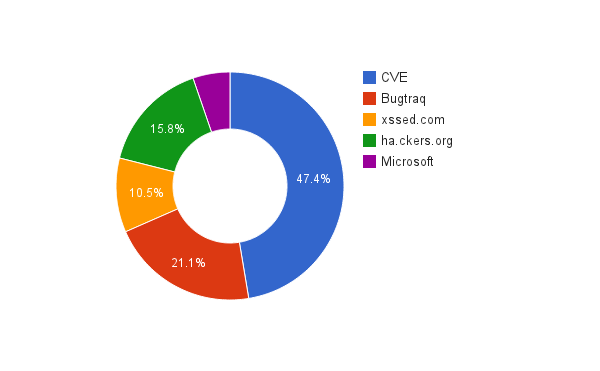
\includegraphics[scale=0.47]{defect-percentages.png}
\end{center}
\caption{\label{fig:defect_sources}A pie showing the sources
where the authors reffered to, to find vulnerabilities to test
their mechanisms. We also provide which source was used
in which publication:
{\sc cve}~\cite{XBS06,NLC07,PMP11,BK04,BV08,JB07,SMS13,WPLKK09,JKK06a,PS11},
{\it Bugtraq}~\cite{PB05,KKVJ06,JEP08},
{\sc xss}ed.com~\cite{NSS06,APKLM10},
ha.ckers.org~\cite{TNH07,PSC09,LV09},
Microsoft~\cite{RDWDE07}.}
\end{figure}

Table~\ref{tab:comp} indicates that the authors of 3 out of 34
(8.8\%) publications, provided complete quadruples.
On the other hand, we see that 4 out of
34 (11.7\%) were not tested at all.
In this cases, all the four elements of the
quadruples are not available ({\sc na}).
An interesting observation is that 10 out of 34
(29.41\%) of the authors performed only attacks
during their tests and did not test their mechanisms
to see if they produce any false alarms. The corresponding
quadruples in this case, are the ones that contain {\sc tp} and
{\sc fn} results but {\sc tn} and {\sc fp} results are not
available ({\sc na}). This stresses the fact that authors
maybe more interested into making sure that
their mechanisms can detect known attacks than seeing how
they respond under normal conditions.
In some occasions (where the number of {\sc tp} results
are not quantified), authors did not mention how many or
which attacks they performed.
Also, in some cases, we observe that even if
the authors report the existence of possible
false positive and negative results, they have not
quantified them ({\sc nq}).

Furthermore, we see that 27 out of
34 mechanisms were tested on real-world applications
known to be vulnerable. The vulnerabilities
associated with these applications are enlisted
in the following providers: the Common Vulnerabilities
and Exposures ({\sc cve})
database,\footnote{\url{https://cve.mitre.org/}}
the {\it Bugtraq}\footnote{\url{http://seclists.org/bugtraq/}}
security mailing list, the
{\sc xss}ed.com\footnote{\url{www.xssed.com}}
security bulletin provider, Microsoft's security
bulletin\footnote{\url{https://technet.microsoft.com/en-us/security/bulletin}}
and the ha.ckers.org\footnote{\url{www.xssed.com}}
security bulletin provider. Figure~\ref{fig:defect_sources}
presents how many (in terms of percentages) and which
(in the figure's caption) authors referred to which source.
In numerous occassions authors performed tests based
on the same applications. For example, 12 mechanisms
were tested on a vulnerable version of
{\sc phpbb}.\footnote{https://www.phpbb.com/}

There are also authors that took a different approach.
For instance, during their initial tests,
Stock et al.~\cite{SLMS14} managed to bypass
the browser-based {\sc xss} filters of the
73\% of 1,602 real-world {\sc dom}-based {\sc xss} vulnerabilities.
These vulnerabilities were actually found during
their previous research~\cite{LSJ13}.
Finally, in the publications that
{\sc amnesia} and {\sc sd}river were presented,
authors managed to break existing application suites
and then test the accuracy of their tools on them.

% Comment 1: Regarding the frameworks that were
% not tested in terms of diagnostic performance
% at all, we see that they are mostly coming from
% the etiological category.

% Comment 2: Note though that implementations
% of etiological mechanisms can actually
% be bypassed.

% Comment 3: The above are some extra findings that
% indicate that there is no standard way to
% test such mechanisms. Perhaps, forming a
% standard way to test such tools in terms
% of diagnostic and computational performance
% would be one of the reasons of adopting them.

\subsection{Availability}

Table~\ref{tab:avail} presents our findings regarding the availability
of the mechanism in terms of source code and corresponding
executables. We also examined the availability of the testbeds
mentioned in the paper. The check mark (\tick) indicates that at some
point in the publication there is a homepage where the reader can
refer to, to download the corresponding software. {\bf AO} (Available
On-line) suggests that the software is available on-line but the
address was not mentioned in the paper, which probably indicates that
the authors made it available after the publication. The question mark
({\bf ?}), indicates that a homepage for the software was given in the
publication but now it is not available.

We see that only 6 out of 34 (17.6\%) of the authors provided a
homepage for their mechanism through their publication and 2 from
these 6 homepages are currently not available. In 5 cases authors made
either the source code or their executables available after their
paper got published. Regarding the availability of test materials, we
see that only 3 out of 34 (8.8\%) authors have currently their
testbeds available on-line.

\subsection{Computational Performance}

Table~\ref{tab:comp} shows for every mechanism its corresponding
overhead. In addition, it indicates if the overhead is applied to the
server-side ({\sc s}), or the client-side ({\sc c}). In almost half of
the approaches, 16 out of 34 (47.05\%), the overhead is provided as a
percentage, while in other cases, 7 our of 34 (20.5\%), the authors
provide the time (in terms of ms) that their mechanisms add to the
normal execution time of the protecting entity. Note that in some
cases, the times of normal executions are not provided,
so it is not possible to move from absolute
time measurements to percentage overheads. In 10 cases (29,4\%), the
overhead was either not available ({\sc na}) or not quantified ({\sc
  nq}). In the case of {\sc php aspis}, its authors indicate that with
their mechanism, the execution time is doubled.

\subsection{Ease of Use}
\label{sec:deploy2}

As we observed in Subsection~\ref{sec:deployment},
there are various reasons why a mechanism could
be difficult to deploy.

Consider the majority of mechanisms coming from
the policy enforcement subcategory. In most cases
developers should modify multiple components
to use each mechanism. Specifically, mechanisms like
BrowserShield, and {\sc beep} require modifications
both on the server and the client side.
Thus, it would be difficult for them to be adopted by
both browser vendors and application developers.
On the other hand, there are cases where the policies
introduced in the server are enforced on the client-side,
via a library embedded in the server's response
(i.e. Blueprint). Such an approach is really convenient
since no modifications are needed on the client.

Extensive modifications in the application's source
code can also be a reason that can make a mechanism
difficult to use. {\sc sql}rand, {\sc amnesia},
mechanisms coming from the parse-tree validation
subcategory and mechanisms coming from the taint
tracking subcategory are such examples.
In the first three cases, programmers should modify every
code fragment that involves the execution of a query.
In the latter case they should also change
all the code fragments that involve user-input handling. 

Finally, even though many of the mechanisms that involve
training are easy to deploy, they have a distinct disadvantage.
When the application is altered, mechanisms like {\sc sd}river
and {\sc xss-guard} require a new training phase is necessary.
However, with the increased adoption of automated testing
and continuous integration frameworks, this phase could be
easily repeated.

\subsection{Security}

While describing the various mechanisms in
Section~\ref{sec:defs}, we observed that some
can be bypassed by attackers that know how they
work.

However, some mechanisms are designed in such a way
so that they can be extended and become immune to
the attacks that they are currently vulnerable to. For
example, policy enforcement frameworks that are
based on JavaScript or {\sc html} rewriting
can be extended to detect attacks that leverage
{\tt iframe} tags (see Subsubsection~\ref{sec:policy}).

This does not apply to all mechanisms though.
In particular, training mechanisms like {\sc didafit},
and {\sc xss-guard} must be redesigned
to detect the attacks that were described in
Subsubsection~\ref{sec:train} and
Subsection~\ref{sec:hybrid} respectively.

\subsection{Point of Detection}

Given the fact that the final steps of
{\sc dsl} injection and {\sc csrf} attacks take place
on the server-side, all the mechanisms that detect
such attacks are placed in some point within the server.
From the mechanisms that detect {\sc dsl} code injection
attacks, 3 out of 13 (23\%) do so at the level
of the {\sc rdbms}---Point {\sc sdb}.
The other 11 wrap {\sc api} calls related to output
vectors---Point {\sc e}i{\sc q}.

In frameworks that deal with JavaScript-driven {\sc xss} attacks we
see that attack detection may take place either on the server-side or
on the client-side. In the first case, a proxy is placed on the server
to examine the server's responses before they reach the user's web
browser. In the second case a modified browser or a library that is
securely downloaded from the server checks the responses for potential
attacks. We find that the tendency so far is to create frameworks that
perform detection on the client side: in particular, 11 out of 19
frameworks (57,8\%) detect JavaScript-driven {\sc xss} attacks on the
client's side. Note that the majority of the mechanisms that detect
such attacks on the server-side can also detect {\sc dsl} code
injection attacks (7 out of 8).

\section{Lessons Learned}
\label{sec:lessons-learned}

% @dimitro: move this to the analysis Section:
% This scheme is an efficient scheme that focuses
% on a specific category of {\sc xss} attacks and
% takes into consideration many attack vectors
% that many of the previous schemes do not.
% Also: 
% As the author of {\sc csse} state~\cite{PB05}, the prevention
% of {\sc xss} attack requires a more complex analysis.

One of our key findings indicate that many detect mechanisms are
tested in a poor manner. In many cases researchers tend not to provide
the false positive and negative results that their tools may produce.
Discussing about the existence of such results and not quantifying
them also blurs the picture.

A reasonable argument would be that many mechanisms (especially the
ones coming from the etiological category), do not need to be
established purely through testing since they provide systematic
arguments as to why their design is secure against attacks. In order
for this to hold, however, an implementation of a defense mechanism
may be entirely correct in terms of its specification, which may not
happen in practice. Moreover, even a mechanism that detects an attack
based on its root cause, instead of observer behavior, may still be
circumvented so that attacks will pass undetected.

When we introduced specicifity and sensitivity in
Section~\ref{ssec:diagnostic-performance} we deferred discussion of
\textsc{ppv} and \textsc{npv} to this point. These two relate to the
performance of a detection mechanism in an actual production setting,
instead of a testbed. If an attack is detected in a production
environment, how much should we be worried? The answer is provided by
\textsc{ppv}. If no attack is detected in a production environment,
how relaxed should we be that no attack has indeed taken place? The
answer is provided by \textsc{npv}. We can calculate \textsc{ppv} and
\textsc{npv} with the following equations:

\begin{equation}
\textsc{ppv} = \frac{\textsc{tp}}{\textsc{tp} + \textsc{fp}}
\end{equation}

\begin{equation}
\textsc{npv} = \frac{\textsc{tn}}{\textsc{fn} + \textsc{tn}}
\end{equation}

\noindent
Equations~\ref{eq:ppv-se-sp} and~\ref{eq:npv-se-sp} use true and false
positives and negatives, like equations~\ref{eq:sensitivity}
and~\ref{eq:specificity}. However, \textsc{tp}, \textsc{tn},
\textsc{fp}, and \textsc{fn} are not the same in the two cases:
whereas sensitivity and specificity are measured on a test
environment, \textsc{ppv} and \textsc{npv} are measured on the real,
target environment. In fact, if \textsc{pr} is the probability of
attacks in the real world, the prevalence, then we
have~\cite{linn2004,altman1994}:

\begin{equation}
\textsc{ppv} = \frac{\textsc{se}\times \textsc{pr}}{
\textsc{se}\times \textsc{pr} + (1 - \textsc{sp})\times (1 -
\textsc{pr})}
\label{eq:ppv-se-sp}
\end{equation}

\begin{equation}
\textsc{npv} = \frac{\textsc{sp}\times (1 - \textsc{pr})}{
(1 - \textsc{se})\times \textsc{pr} + \textsc{sp}\times (1 -
\textsc{pr})}
\label{eq:npv-se-sp}
\end{equation}

\noindent
The prevalence is the prior probability that an event is an attack,
based on our understanding of the volume and frequency of attacks; the
\textsc{ppv} and \textsc{npv} are the revised estimates of the
probability based on the results of the detection
mechanism~\cite{altman1994}. The lower the prevalence of an attack,
the more confident we can be that a negative test result indicates
that no attack has taken place and the less sure we can be that a
positive test result indicates a real attack. 

Of course it is not easy, and it may not even be possible, to know how
prevalent an attack is. Also, attacks on a system may depend on
factors such as its visibility and popularity, so that the same piece
of software may be subject to varying attack regimes depending on
where it is actually deployed. With this in mind it may be unfair to
ask of researchers to provide \textsc{ppv} and \textsc{npv} values for
their mechanisms---in fact, we see that nobody does.

That does not mean that deriving \textsc{ppv} and \textsc{npv} is
altogether impossible. One could deploy a system, armoured with an
attack detection mechanism, on a honeypot to study what happens over
a length of time. This could give an indication of the performance of
the mechanism out in the wild. Alternatively, one could deploy a
target, unarmoured system, on a honeypot to study the prevalence of
the class of attacks to be detected. Studying the prevalence of
classes of attacks could be an interesting area of study on its own,
which could feed directly on the evaluation of attack detection
mechanisms as practical tools.

Apart from demonstrating the value of a mechanism, good accuracy tests
may be beneficial per se, by leading to more well-designed and robust
mechanisms. Mechanisms that can be circumvented were not extensively
tested in terms of accuracy. For instance, {\sc didafit} was not
tested at all and {\sc xss-guard}'s testing involved 6 known attacks.
This also applies to some frameworks coming from the taint tracking
subcategory. It is possible that more tests during development would
have led the authors to wider improvements in design. 
%% PL: Do we have a reference in Software Engineering correlating
%% testing with better design?

The accuracy of a tool may be related to the scope of the attacks it
aims to detect. A more limited scope may allow the development of more
accurate tools. In this vein, the system by Stock et al~\cite{SLMS14}
is the only one that targets exclusively {\sc dom}-based {\sc xss}
attacks and detects them in an accurate manner as seen in
Table~\ref{tab:comp}. It is also extensively tested in real-world
attacks.

Apart from testing practices, another area that merits improvement is
the availability of source code and testbeds. We are not aware of
specific reasons why authors of attack detection mechanisms seem to be
wary of releasing online their code and tests. Our finding may reflect
the status in the current point in time, when authors are urged to
publish their code and tests, and may start, or may have already
started doing so, but this does not show yet in the research we
examined, which goes several years back. We also saw instances where
material was published, but does not seem to be available any more.
That points to the importance of curation of research materials. That
is a problem arising in all scientific fields. It is not enough to
publish the underlying code and data, but to make sure that it remains
accessible and to provide the means to test it even as technology
progresses and operating systems, file formats, and software libraries
change. That may be too much to ask right now; what seems reasonable,
though, is to ask of researchers in attack detection mechanisms not to
buck the trend and to take steps to increase the availability of their
research.

Another interesting finding involves the computational overhead. We
observe that the average overhead that can be extracted from the
publications that provide the overhead in percentage terms is 18\%.
Relative research on protection mechanisms~\cite{SPWS13} indicates
that mechanisms that introduce an overhead larger than 10\% do not
tend to gain wide adoption in production environments. Hence, the
computational overhead of some mechanisms could be a reason why they
have not been adopted.

We need to mention that the fact that mechanisms come
sometimes with deployment difficulties does
not necessarily mean that this is a serious reason
not to adopt them. The deployment of such frameworks
is most of the time complex because as we observed
in Section~\ref{sec:attacks} the attacks that they
detect are complex too. So every security feature can
come with such a trade-off and those who intend to use it
should be aware of this.

Deployment can also depend on the detection point
of an attack. We saw that many policy enforcement
mechanisms that detect attacks at Point {\sc ub},
are not easy to deploy because modifications
are needed both on the server and the client side.
We observed though that Blueprint has not such
deployment issues (see Subsection~\ref{sec:deploy2}).
Thus, when developing a new countermeasure,
researchers should consider where they are planning
to detect attacks, observe the corresponding
deployment challenges, and try to mitigate them.

% discuss Availability. Finally, 

\section{Conclusions}
\label{sec:conclusion}

Despite many approaches that have been developed,
application attacks based on source code injection
have been consistently present for the last 15 years,
and it appears that they will continue to be.
Attackers seem to find new ways to introduce
source code to applications by using a variety of
languages and techniques~\cite{HNSHS12,DKH14}.
Meanwhile, during the last decade, there are
numerous mechanisms that have been developed to
detect one or more of such attacks. However,
% even if
% some of them share characteristics with supported frameworks
% like Mozilla's Content Security
% Policy\footnote{\url{https://developer.mozilla.org/en-US/docs/Web/Security/CSP}}
% ({\sc csp}) and Google
% Caja\footnote{\url{https://code.google.com/p/google-caja/}}~\cite{M06},
the majority of them are not used in practice.

In this paper we first introduced an exploitation model
that can be a reference point which can be used by
researchers who wish to develop new countermeasures.

% This is due to the following reasons:
% a) the mechanisms have not been extensively tested in terms
% of accuracy,
% b) are hard to deploy because they require many modifications
% either on the client-side, the server-side, or both,
% c) they add significant overhead, and
% d) can be bypassed by attackers that know how they work.
% The motivation behind this research is to systematize
% and analyze previously proposed protection mechanisms.
% In this way we can highlight the advantages
% and disadvantages of each mechanism, enlist them
% into different categories, and see how they compare to each other.

\begin{itemize}
\item We believe that our research may facilitate researchers
or practitioners who would like to use one of the
aforementioned mechanisms and researchers who would like
to build new ones. Especially in the second case,
researchers can utilize our exploitation model as a
starting point to develop their approach.
\item We believe that forming a
standard way to test such mechanisms in terms
of accuracy and computational performance
would be one of the reasons of adopting them.
\end{itemize}

\bibliographystyle{IEEEtran}
\bibliography{questioning}

\end{document} 

